\subsection{$k$-Nearest Neighbors}

The $k$-nearest neighbors algorithm ($k$-NN) is a nonparametric method commonly used for classification, where each object is classified by a vote among its $k$ nearest neighbors.\cite{altman1992introduction} Since the algorithm is substantially a local method, it would be less likely to be influenced by global topology of the attribute space, which suggests an important advantage of applying $k$-NN here.

However, it is also noteworthy that the $k$-NN algorithm suffers from severe curse of dimensionality. What makes it worse is that we have got only 2192 observations here but more than 10 attributes. Therefore some variable selection must be applied before launching the $k$-NN algorithm.

\begin{figure}[h]
\center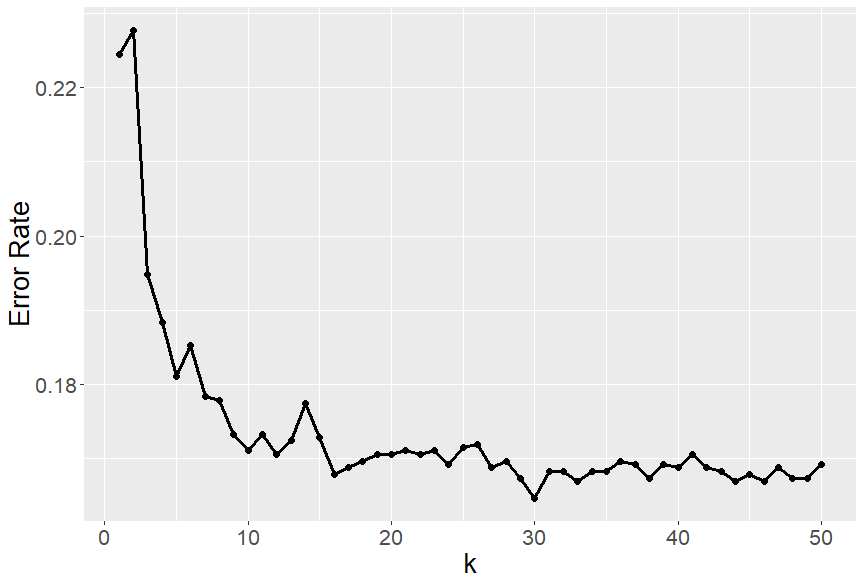
\includegraphics[width = .7\textwidth]{knncv.png}
\caption{Cross Validation Error Rates of \(k\)-NN}
\label{knncv}
\end{figure}

\begin{table}[h]
\setlength{\belowcaptionskip}{5pt}
\caption{Confusion Matrix and Error Rates of \(k\)-NN}
\label{errknn}
\centering
\renewcommand\arraystretch{1.5}
\begin{tabular}{rrrrr}
\hline
\hline
 & & \multicolumn{2}{c}{True Condition} & \\
\hline
 & & Non-Precipitation & Precipitation & \\
\cline{1-4}
\multirow{2}{*}{Prediction} & {Non-Precipitation} & 308 & 52 & \\
\cline{2-4}
&Precipitation&58&241&\\
\hline
&Error Rate & 0.1585 & 0.1775 & 0.1669\\
\cline{2-5}
& & Type \uppercase\expandafter{\romannumeral1} & Type \uppercase\expandafter{\romannumeral2} & Overall\\
\hline
\end{tabular}
\end{table}

Fortunately, the process of variable selection can be done with the result of the random forest which we have launched before. According to random forest, the most important attributes are PRCP, TDIF, and the four attributes regarding wind.

The data set can be even further reduced as we observe the strong correlation between WSF2 and WSF5 (their correlation turns out to be approximately $0.95$). Because of such stong colinearity, we would only keep 4 attributes, i.e. PRCP, TDIF, WSF5 and WDF5 in the $k$-NN algorithm. (Note that for wind vectors, the distances shall not be Euclidean as they are presented in polar coordinates.)

The cross validation error rates for different values of $k$ are shown above in Figure \ref{knncv}, which suggests that $k=30$ would be the best to proceed with. Then the confusion matrix and the test errors are as follows in Table \ref{errknn}.

As we can see, in general, SVM has the best performance, while $k$-NN the worse. It is also noteworthy that for all of the three methods here, there are always more Type \uppercase\expandafter{\romannumeral2} error than Type \uppercase\expandafter{\romannumeral1} error.

